\documentclass[12pt, letterpaper]{article}
\usepackage[utf8]{inputenc}

\usepackage{pdfpages}
\usepackage{graphicx}
\graphicspath{{images/}}

\title{\textbf{Module Guide for Bomber Clone Application \\ \Large Software Engineering 3XA3: Project}}
\author{Group 12 - The A Team \\Gabriel Lopez De Leon, 1310514\\Ren-David Dimen, 1222679\\Jay Nguyen, 1327828}
\date{06 November 2015}

\renewcommand*\contentsname{Table of Contents}
\setcounter{tocdepth}{4}
\setcounter{secnumdepth}{4}

\begin{document}
	
	\begin{titlepage}
		\clearpage\maketitle
		\thispagestyle{empty}
	\end{titlepage}
	
	\newpage
	\tableofcontents
	\newpage
	
	\section{Revision History}
	
	\begin{tabular}{ |c|c|c|c| } 
		\hline
		\textbf{Revision \#} & \textbf{Revision Date} & \textbf{Description of Change} & \textbf{Author}\\
		\hline
		6 & Nov 06 2015 & Added Section 8 & Ren-David Dimen\\
		\hline
		5 & Nov 06 2015 & Added Section 9 & Gabriel Lopez de Leon\\
		\hline
		4 & Nov 05 2015 & Added Section 4, 6, 7 & Gabriel Lopez de Leon\\
		\hline
		3 & Nov 02 2015 & Added Section 5 & Ren-David Dimen\\
		\hline
		2 & Nov 02 2015 & Added Section 1 and 2 & Gabriel Lopez de Leon\\
		\hline
		1 & Nov 02 2015 & Added Section 3 & Ren-David Dimen\\
		\hline
	\end{tabular}
	
	\newpage
		
	\section{Introduction}
	\indent \indent Our project is the recreation of a game called Bomberman, we are taking legacy code for a game very similar to the original and reimplementing it with proper code structure and documentation. Our Software Requirements Specification (SRS) document and Test Plan describe how we are planning on implementing the game and how it will be tested through the use of manual and automated tests. The game overall will have the same objectives as the original, to eliminate other players by placing bombs in the arena. We will be using threads in the implementation of the game and instead of using 2D arrays or an arena divided into tiles, we plan to use pixels for hit detection to make the game look and feel more smooth as it is played. To test the various functional and non-functional requirements we will be using black box, white box and unit testing as aforementioned in our Test Plan. \\
	 
	While the SRS focuses on the "what", the Design document focuses on the "how." The design documentation for our project is divided into the Module Guide (MG) and the Module Interface Specification (MIS). This document will focus on the MG specifically and will show the decomposition of the system into smaller subsections which can be discussed in further detail while also showing how these different modules all relate to one another. This decomposition of a system is a commonly accepted approach in software development. One of the design principles we want to use is Information Hiding. This supports design based on change as the various "secrets" each module hides is equivalent to anticipated changes. Having a design follow this principle allows for quick and easy modification of code which we had already anticipated would change. Furthermore, there is a set structure to the code, parts that are unlikely to change a group together while as the once subject to likely change in the future are also grouped together. \\
	
	\noindent The rest of the document will be organized as follows: \\
	- Section 2 will list the anticipated and unlikely changes in the system. \\
	- Section 3 will summarize the module decomposition based on likely future changes. \\
	- Section 4 will specify the relation between requirements and the modules. \\
	- Section 5 will be describing each module in further detail. \\
	- Section 6 will show traceability matrices for relations between modules and requirements, and between modules and anticipated changes. \\
	- Section 7 will describe the relationships between the modules. \\
	
	\section{Anticipated and Unlikely Changes}
	
	This section lists possible changes within the program according to the likeliness of the change. Possible changes are classified into two different categories.
	
	\subsection{Anticipated Changes}
	
	Anticipated changes are the source of the information that is to be hidden inside the modules. Ideally, changing one of the anticipated changes will only require changing the one module that hides the associated decision. The approach adapted here is called design for change.\\
	
	\textbf{AC1:} The data structure in which the state of the board is saved.\\
	
	\textbf{AC2:} The initial state of the board.\\
	
	\textbf{AC3:} Character states.\\
	
	\textbf{AC4:} How the program's state is displayed.\\
	
	\textbf{AC5:} Character hit-box size.\\
	
	\textbf{AC6:} Window output size.
	
	\subsection{Unlikely Changes}
	
	Modules with unlikely changes may not inherently follow the norms of information hiding. Interacting modules may need to be updated if one or more module is modified, therefore these changes must be dealt with care so as to not negatively affect the outcome of the program.\\
	
	\textbf{UC1:} Input hardware devices. (ie keyboard and mouse)\\
	
	\textbf{UC2:} Output hardware devices. (ie monitor)\\
	
	\textbf{UC3:} User control inputs. (up, down, left, right arrow keys, etc.)\\
	
	\textbf{UC4:} Data type of the character sprites.
	
	\section{Module Hierarchy}
	This section provides an overview of the module design. Modules are summarized in a hierarchy decomposed by secrets in Table 1. The modules listed below are the modules which will be implemented.\\
	
		\textbf{M1:} Hardware-Hiding Module\\
		
		\textbf{M2:} Screen Module\\
		
		\textbf{M3:} Sprite Module\\
		
		\textbf{M4:} SpriteSheet Module\\
		
		\textbf{M5:} Keyboard Module\\
		
		\textbf{M6:} Player Module\\
		
		\textbf{M7:} CollisionTest Module
	
	\begin{center}
		\begin{tabular}{ p{6cm} p{4cm} p{4cm}  }
			\hline
			\textbf{Level 1} & \textbf{Level 2} & \\ 
			\hline
			Hardware-Hiding Module \\ 
			\hline 
			Behaviour-Hiding Module & Screen Module &   \\ 
			& Sprite Module & \\
			& SpriteSheet Module & \\
			& Keyboard Module & \\
			& Player Module & \\

			\hline
			Software Decision Module & CollisionTest Module &   \\ 
			\hline
			
		\end{tabular}				
		\footnotesize Table 1: Module Hierarchy
	\end{center}
	
	\section{Connection Between Requirements and \\ Design}
	
	\indent \indent The design of the system is intended to satisfy the requirements developed in the SRS. In this stage, the system is decomposed into modules. The connection between requirements and modules are listed in section 7, Traceability Matrix.\\
	
	\section{Module Decomposition}
	
	\indent \indent Modules are decomposed following the principle of "information hiding" which was proposed by David Parnas. The secrets listed within the module decomposition will provide information on the design decision hidden by its respective module. The "service" section will be describing what each module does without specifying how it will do it. For each of the following modules, a suggestion for the implementation software used is given under the section "Implemented By." An entry of OS refers to modules provided by the operating system/standard programming language libraries and a dash (-) means the module will not have to be implemented.
	
	\subsection{Hardware Hiding Modules (M1)}
	\noindent \textbf{Secrets:} The data structure and algorithm used to implement the virtual \indent hardware.\\
	
	\noindent \textbf{Services:} Serves as virtual hardware used by the rest of the system. This \indent module provides the interface between the hardware and the software. \indent So, the system can use it to display outputs or to accept inputs.\\
	
	\noindent \textbf{Implemented By:} OS
	
	\subsection{Behaviour-Hiding Module}
	\noindent \textbf{Secrets:} The contents of the required behaviours.\\
	
	\noindent \textbf{Services:} Includes programs that provide externally visible behaviour of \indent the system as specified in the software requirements specification (SRS) \indent document. This module serves as a communication layer between the \indent hardware-hiding module and the software decision module. Programs in \indent this module will need to change if there are changes in the SRS.\\
	
	\noindent \textbf{Implemented By:} - 
	
	\subsubsection{Screen Module (M2)}
	\noindent \textbf{Secrets:} The format and structure of the display (output) data.\\
	
	\noindent \textbf{Services:} This module is used to render images and output them into a \indent display.\\
	
	\noindent \textbf{Implemented By:} Eclipse
	
	\subsubsection{Sprite Module (M3)}
	\noindent \textbf{Secrets:} The format and structure of the sprites (input) used.\\
	
	\noindent \textbf{Services:} Obtains the sprites from a set path and uses them for different \indent character actions/movement.\\
	
	\noindent \textbf{Implemented By:} Eclipse
	
	\subsubsection{SpriteSheet Module (M4)}
	\noindent \textbf{Secrets:} The format and structure used to obtain the sprite sheet.\\
	
	\noindent \textbf{Services:} Sets the main path to the sprite sheet which will be loaded and \indent used in other modules.\\
	
	\noindent \textbf{Implemented By:} Eclipse
	
	\subsubsection{Keyboard Module (M5)}
	\noindent \textbf{Secrets:} The format and structure of user input.\\
	
	\noindent \textbf{Services:} Takes input date from keyboard keys and converts it to data to \indent be used by other modules.\\
	
	\noindent \textbf{Implemented By:} Eclipse
	
	\subsubsection{Player Module (M6)}
	\noindent \textbf{Secrets:} The format and structure of the player entity.\\
	
	\noindent \textbf{Services:} Links input data to the player sprite.\\
	
	\noindent \textbf{Implemented By:} Eclipse
	
	\subsection{Software Decision Module}
	\noindent \textbf{Secrets:} Design decisions based on mathematical theorems, physical facts, \indent or programming considerations are found here. The various secrets of this \indent module are not described in the SRS.\\
	
	\noindent \textbf{Services:} Includes data structure and algorithms used in the system that \indent do not provide direct interaction with the user.\\
	
	\noindent \textbf{Implemented By:} -
	
	\subsubsection{CollisionTest Module (M7)}
	\noindent \textbf{Secrets:} The format and structure of the object states in the game.\\
	
	\noindent \textbf{Services:} Handles the collision detection (hit tests) between objects.\\
	
	\noindent \textbf{Implemented By:} Eclipse
	
	\section{Traceability Matrix}
	This Section shows traceability matrices between modules and requirements, and between modules and anticipated changes. Note that requirements R1 to R5 are listed on the SRS.
		\begin{center}
			\begin{tabular}{ p{6cm} p{4cm} p{4cm}  }
				\hline
				Req. & Modules &\\ 
				\hline
				R1  & M2, M7 & \\ 
				R2  & M2 & \\
				R3  & M2, M3, M4 & \\
				R4  & M5 & \\
				R5  & M6 & \\
				\hline
				
			\end{tabular}				
			\footnotesize Table 2: Trace Between Requirements and Modules
		\end{center}
		
				\begin{center}
					\begin{tabular}{ p{6cm} p{4cm} p{4cm}  }
						\hline
						AC. & Modules &\\ 
						\hline
						AC1  & M7 & \\ 
						AC2  & M2 & \\
						AC3  & M6 & \\
						AC4  & M4 & \\
						AC5  & M3 & \\
						AC6  & M1 & \\
						\hline
						
					\end{tabular}				
					\footnotesize Table 3: Trace Between Anticipated Changes and Modules
				\end{center}
	
	\section{Use Hierarchy Between Modules}
	
	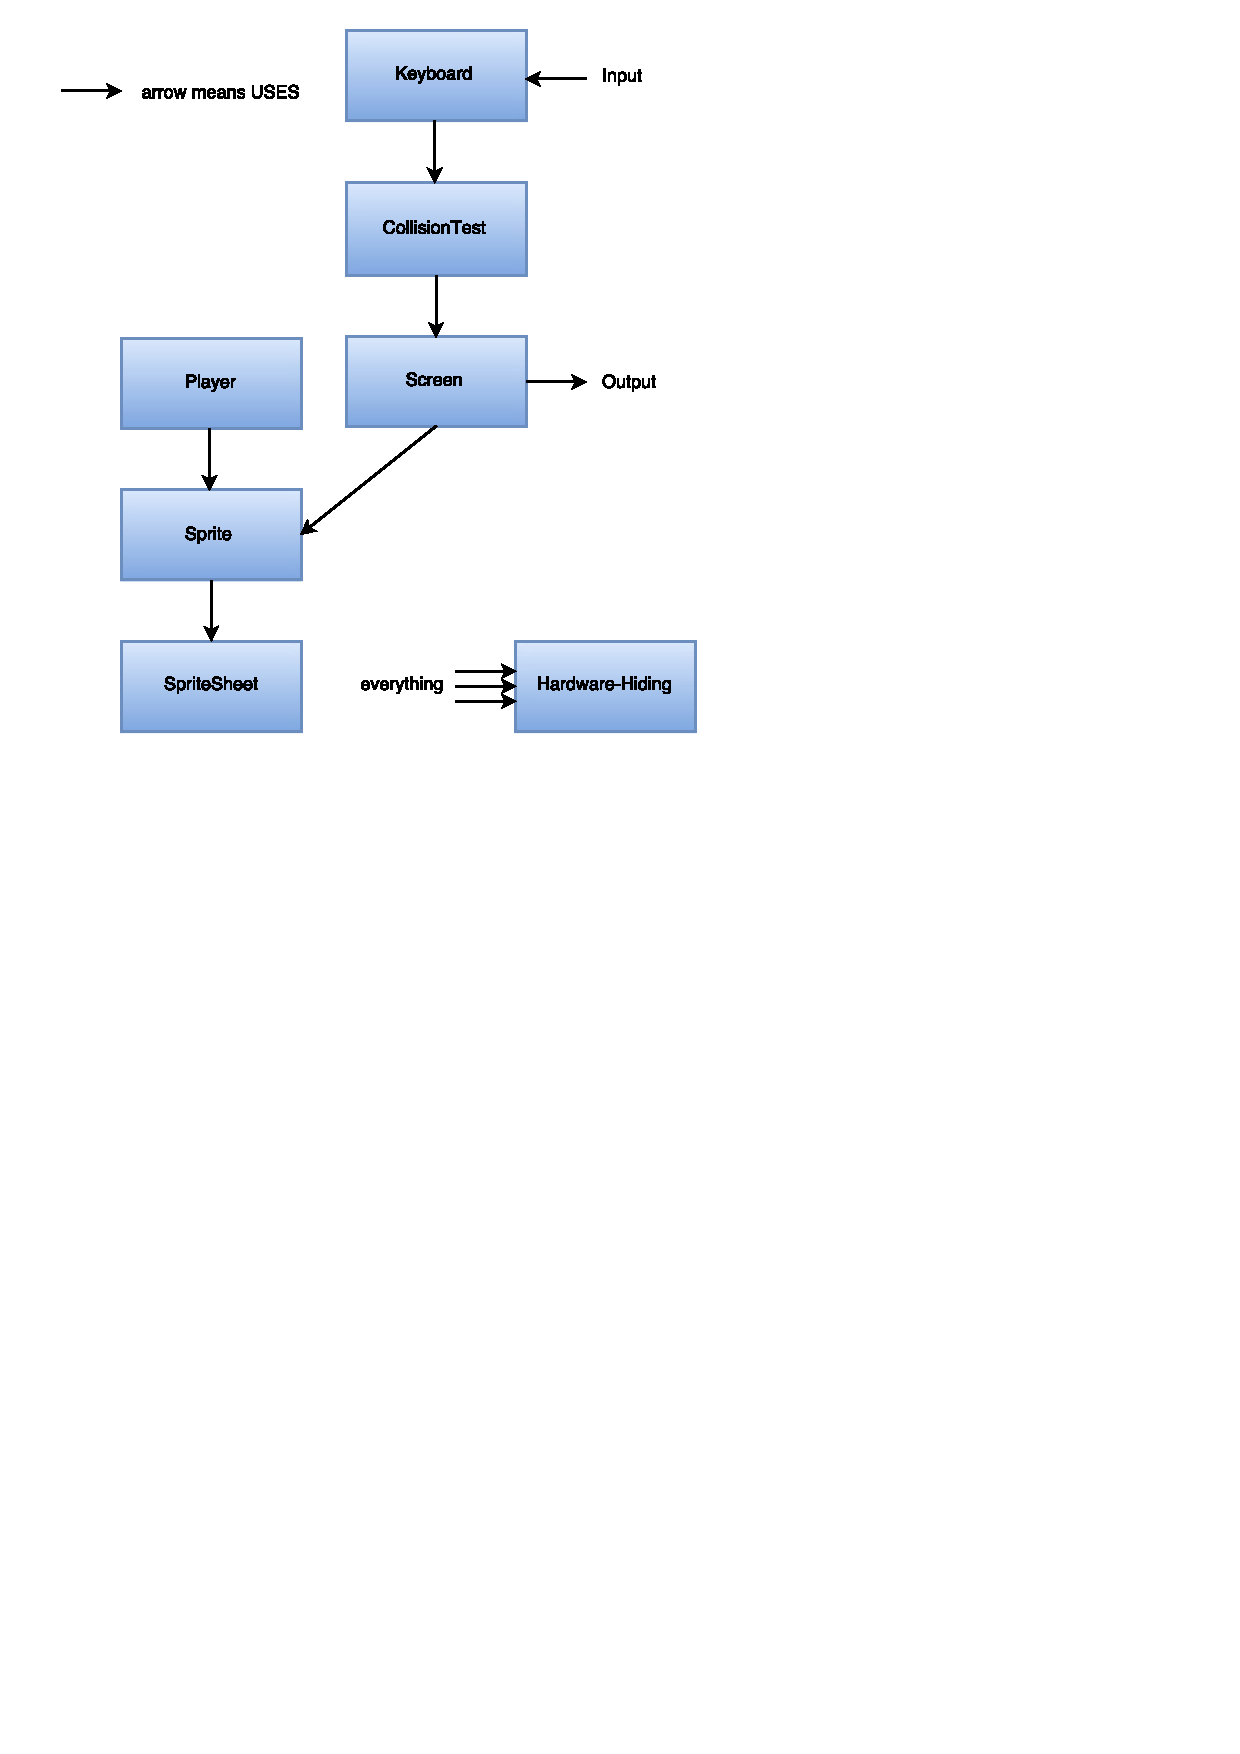
\includepdf{useHierarchy.pdf}
	
	\section{Schedule}
	\subsection{Milestones} 
	Note that these milestones also appear on the Gantt and Pert charts found in the design document folder in the repository.\\
	
	\noindent A. \indent \indent testing - to be completed by November 25, 2015 \\
	\noindent B. \indent \indent Test Report Revision 0 - November 27, 2015 \\
	\noindent C. \indent \indent Complete implementation of code - complete by November 27, 2015 \\
	\noindent D. \indent \indent Final Demonstration Revision 1 - November 30 - December 4, 2015 \\
	\noindent E. \indent \indent Final Documentation Revision 1 - December 8, 2015 \\
	
	\subsection{Gantt Chart}
	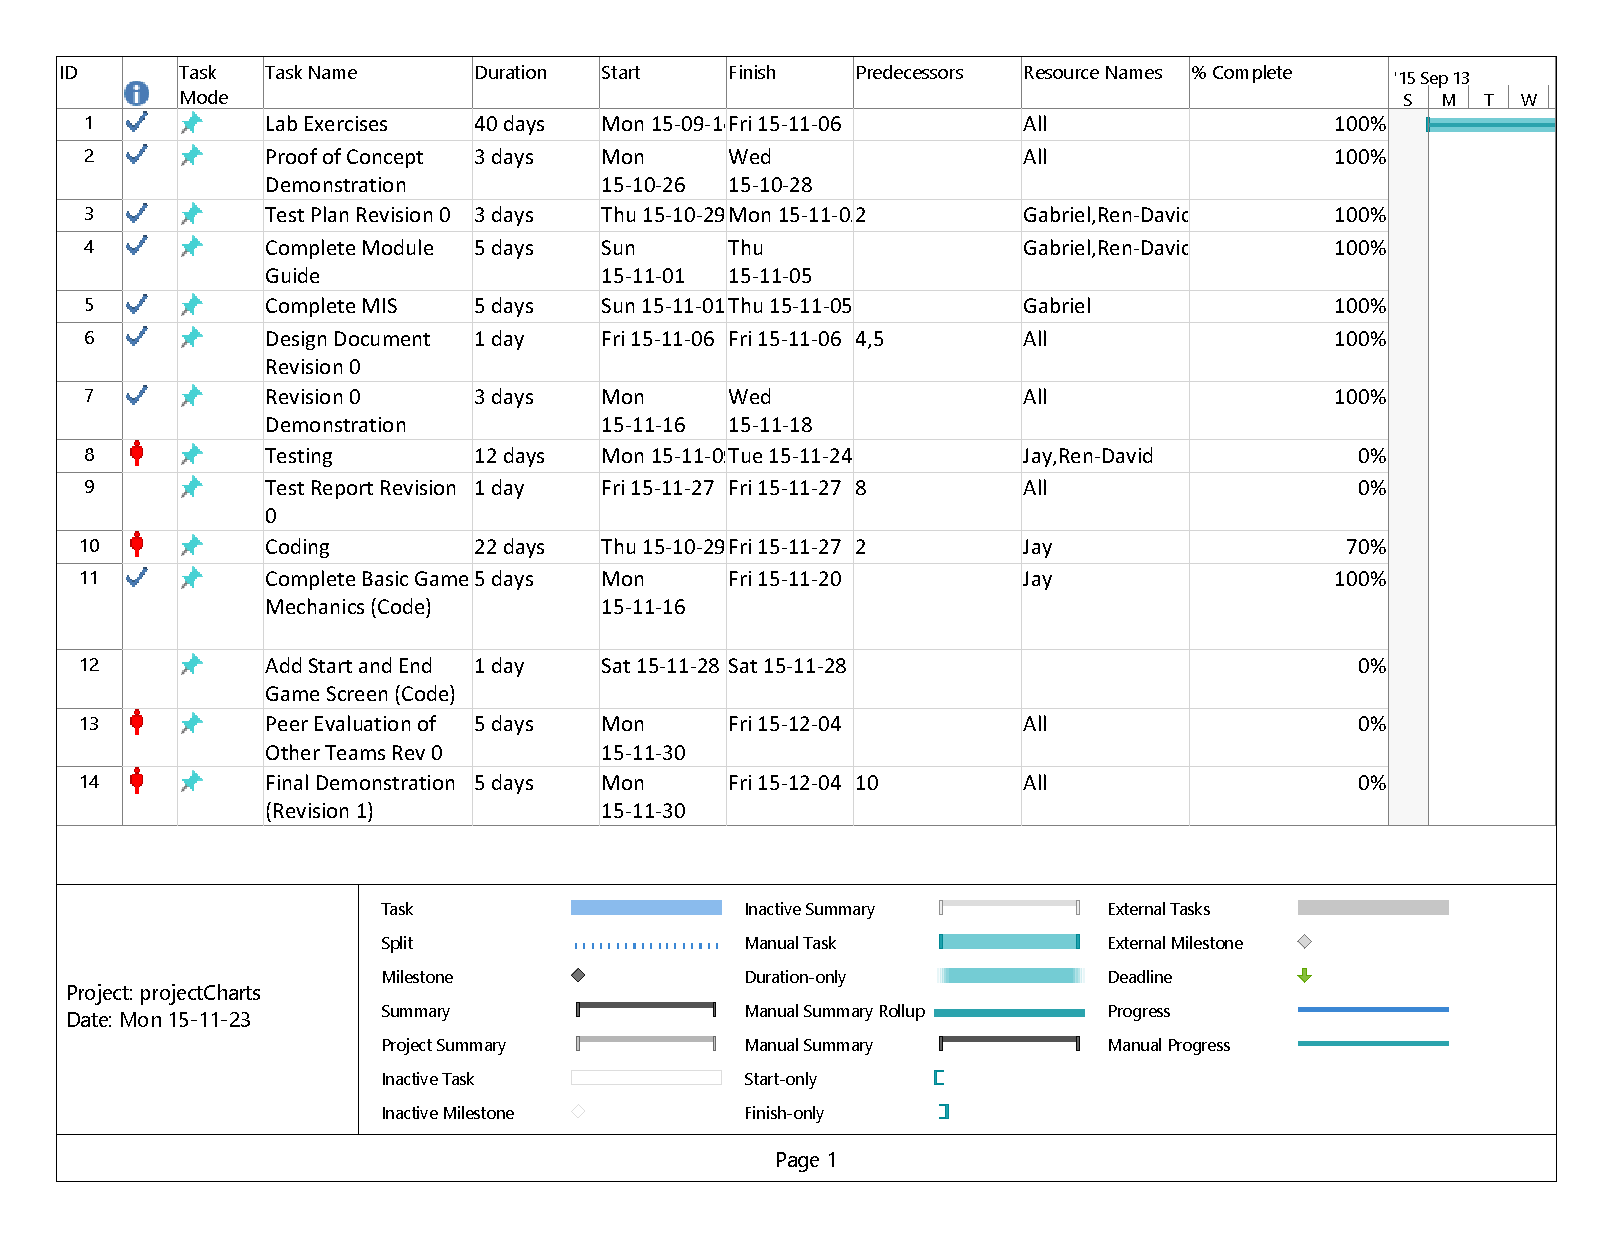
\includepdf[pages=-]{projectGantt.pdf}
	
	\subsection{Pert Chart}
	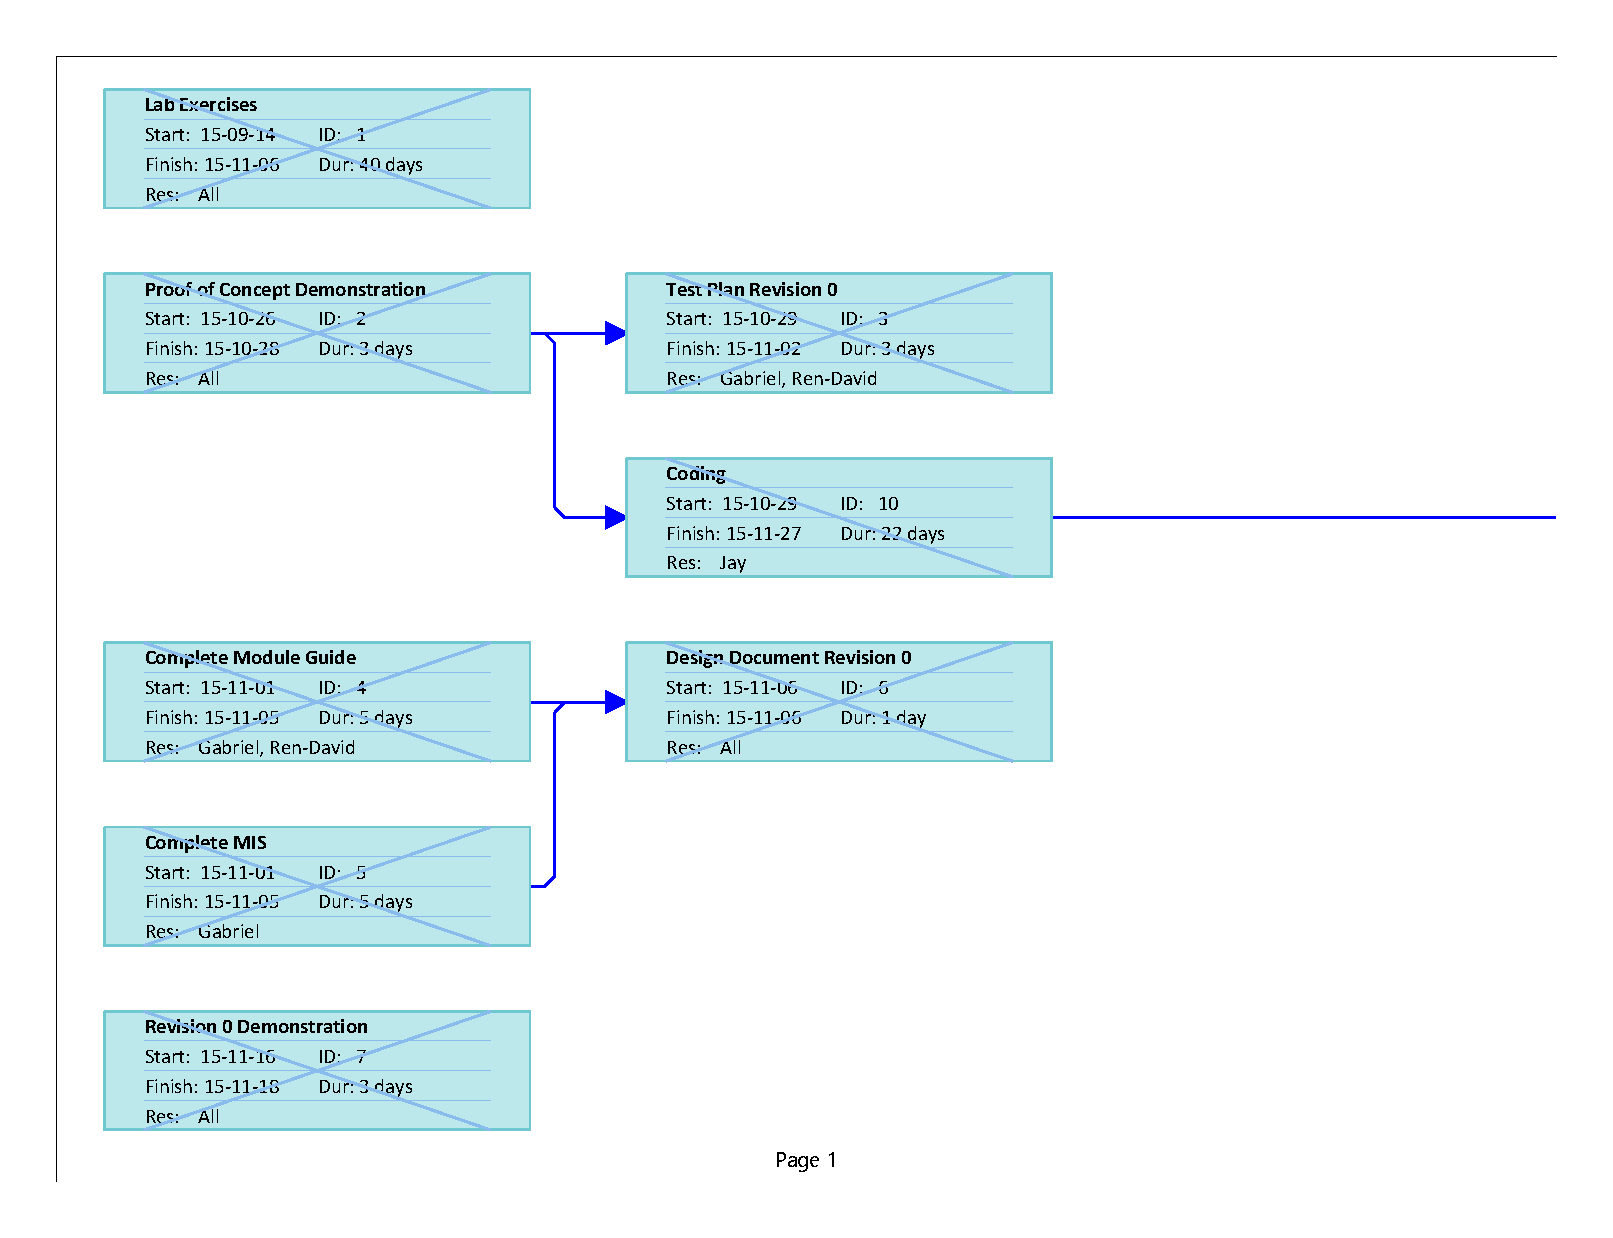
\includepdf[pages=-]{projectPert.pdf}
	
	
\end{document}